\documentclass[12pt]{article}

\usepackage[french]{babel} % Document en français
\usepackage[T1]{fontenc} % Suppression d'un warning
\usepackage[utf8]{inputenc} % Document UTF8
\usepackage{graphicx} % Insertion d'images
\usepackage[left=2.2cm, right=2.2cm, top=2.5cm, bottom=2.5cm]{geometry} % Mise en page
\usepackage{multicol} % Texte en multicolonnes avec multicols
\usepackage{placeins}
\usepackage{titling}

\graphicspath{{res/}}

\newcommand{\HRule}{\rule{\linewidth}{0.5mm}}

\begin{document}

\begin{titlepage}
\begin{center}

% Upper part of the page. The '~' is needed because \\
% only works if a paragraph has started.

\includegraphics[width=0.15\textwidth]{./logo_ucl.png}~\\[1cm]

\textsc{\LARGE Université Catholique de Louvain}\\[1.5cm]

\textsc{\Large Notes de cours}\\[0.5cm]

% Title
\HRule \\[0.4cm]
{ \huge \bfseries LECGE1321 - Management humain \\[0.4cm] }

\HRule \\[1.5cm]

% Author and supervisor
\noindent
\begin{minipage}[t]{0.4\textwidth}
\begin{flushleft} \large
\emph{Auteur:}\\
Florian \textsc{Thuin} \\
Eddy \textsc{Ndizera}
\end{flushleft}
\end{minipage}%
\begin{minipage}[t]{0.4\textwidth}
\begin{flushright} \large
\emph{Professeur :} \\
Nathalie \textsc{Delobbe}
\end{flushright}
\end{minipage}

\vfill

% Bottom of the page
{\large \today}

\end{center}
\end{titlepage}

%\maketitle
\tableofcontents

\section{Introduction}
  \subsection{Le champ du management humain}
  \subsection{Cas type : France Telecom}
  \subsection{Un outil d'analyse : les niveaux d'Ardoino}
  Les niveaux d'intelligibilité d'Ardoino sont un modèle d'analyse d'une réalité sociale. Celui-ci permet de mettre en défaut la pensée simpliste qui consiste à attribuer une erreur à un facteur individuel (\og{} erreur fondamentale d'attribution\fg{}). La théorie fondamentale de l'attribution consiste d'une part à attribuer sa propre réussite à soi-même et ses échecs à un contexte et d'autre part à attribuer la réussite des autres à un contexte et leurs échecs à eux-mêmes.
  
  Il y a 5 niveaux :
  
  \begin{enumerate}
   \item Le niveau individuel
   \item Le niveau relationnel et groupal
   \item Le niveau organisationnel
   \item Le niveau institutionnel
   \item Le niveau d'historicité
  \end{enumerate}
  
  % TODO : Include l'image du modèle d'Ardoino
  
  \begin{description}
   \item[Niveau individuel] : les facteurs individuels d'ordre psychologiques (attitude, caractère, personnalité, motivations,...)
   \item[Niveau relationnel et groupal] : les relations interpersonnelles et affectives (la communication). Ce niveau étudie les phénomènes de groupe : cohésion, appartenance, esprit de groupe, amitié, complicité, conflits interpersonnels.
   \item[Niveau organisationnel] : les modalités d'organisation de l'action collective. Ce niveau étudie les problèmes d'efficacité : les règles, lee rôles, les status, les modes de division et de coordination du travail, la structure du pouvoir,... 
   \item[Niveau institutionnel] : les valeurs, les normes, la culture. Ce niveau étudie les institutions publiques, les cadres politique, juridique, social et économique ainsi que les règles formelles (lois) et informelles (culture, traditions) qui régissent l'ensemble de la société.
   \item[Niveau d'historicité] : analyse des autres dimensions à travers l'histoire. Ce niveau étudie les transformations de la société, les mouvements sociaux, les tendances économiques, les rapports de force entre les classes sociales,...
  \end{description}
  \subsection{Management humain : de quoi parle-t-on ?}
    \subsubsection{People management}
      Le people management correspond à l'encadrement des employés et au leadership par différents moyens :
      
      \begin{itemize}
       \item Organisation et coordination du travail
       \item Supervision et développement des individus
       \item Animation et conduite des équipes
      \end{itemize}
    
    \subsubsection{Gestion des ressources humaines}
      
      La gestion des ressources humaines est plus formalisée et a pour thèmes :
      
      \begin{itemize}
       \item Le recrutement et la sélection
       \item L'allocation et la planification des ressources humaines
       \item La classification des emplois et les rémunérations
       \item Le développement des employés et les formations
       \item L'évaluation des performances
       \item Le dialogue social et la communication
      \end{itemize}
      
  \subsection{Le modèle de Kolb}
  
  L'activité d'un manager dans les RH peut être représentée par le modèle de Kolb.
  
  % TODO : Insérer le modèle de Kolb
  
  \subsection{Structure générale du cours}
    Le cours se partage en deux axes.
    
    \paragraph{Axe historique}
      \begin{enumerate}
       \item L'administration du personnel
       \item L'école des relations humaines
       \item Le courant socio-technique
       \item La gestion stratégique des ressources humaines
      \end{enumerate}
    
    \paragraph{Axe thématique}
      \begin{enumerate}
       \item L'engagement et la motivation au travail
       \item Le pouvoir, l'autorité et le leadership
       \item La dynamique et les facteurs d'efficacité dans les groupes et équipes
       \item Les valeurs et la culture dans les organisations
      \end{enumerate}

\section{Panorama historique et rôles de la fonction RH}
	\subsection{Les étapes historiques}
	  \begin{itemize}
	   \item Contextes socio-économiques distincts
	   \item Modèles dominants d'organisation du travail et de pensée stratégique
	   \item Conceptions sous-jacentes de l'être humain
	   \item Rôles distincts pour la fonction RH
	   \item Champs de préoccupations et de pratiques RH
	  \end{itemize}
	  
	  \subsection{Les 4 rôles RH (D. Ulrich, 1993)}
	  
	  \begin{enumerate}
	   \item Expert administratif
	   \item Champion des employés
	   \item Agent de changement
	   \item Partenaire stratégique
	  \end{enumerate}

	  % TODO : Include la représentation des rôles RH Ulrich
	  
	  \begin{description}
	   \item[Expert administratif] : rôle centré sur la surveillance des contrats de travail et des règlements (processus et résultats)
	   \item[Champion des employés] : rôle centré sur la motivation des employés (la personne et son développement).
	   \item[Agent de changement] : rôle centré sur l'adaptation et l'évolution de l'organisation et des hommes (stratégies, approche socio-technique)
	   \item[Partenaire stratégique] : rôle centré sur la plus-value et les succès stratégiques de l'organisation (processus et résultats)
	  \end{description}
	  
	\subsection{L'administration du personnel}
	Les fondements de la fonction RH
	  \subsubsection{Le contexte socio-économique}
	  On est en pleine révolution industrielle (18-19ème siècle) dont les principales caractéristiques sont :
	  
	  \begin{itemize}
	   \item Progrès technologique : le machinisme, l'industrialisatio massive de la production ;
	   \item Disparition des corporations de métiers ;
	   \item Patron arbitraire, paternaliste ;
	   \item Avènement de l'entreprise capitaliste ;
	   \item Construction d'un marché de libre échange ;
	   \item Naissance des valeurs démocratiques républicaines ;
	   \item Dualisation de la société : bourgeoisie industrielle VS prolétariat
	   \item Perte d'autonomie et déqualification progressive des travailleurs
	   \item Conditions de travail misérables et précarisation économique de la classe ouvrière
	  \end{itemize}
	  
	  Cette période correspond également la naissance du mouvement ouvrier et du syndicalisme : nouvelle législation et apparition de la concertation sociale.

	  \subsubsection{Les modèles d'organisation du travail}
	  
	  \paragraph{L'organisation scientifique du travail (Taylorisme)}
	  \begin{description}
	   \item[Standardisation] : parcellisation et simplification des tâches (chronométrage des temps et mouvements).
	   \item[Distinction conception-exécution] : pour augmenter le rendement et la qualité de vie des ouvriers.
	  \end{description}
	  
	  \paragraph{Bureaucratie Wéberienne}
	  \begin{description}
	   \item[Formalisation et impersionnalité] : la règle remplace la tradition et l'arbitraire
	   \item[Centralisation et hiérarchisation] : structure hiérarchique conforme au principe d'unité de commandement (= un agent ne doit recevoir des ordres que d'un seul chef)
	  \end{description}
	  
	  \subsubsection{Les options stratégiques}
	  \begin{description}
	   \item[Fordisme] : gains en productivité et croissance assurés par une production et une consommation de masse.
	   \item[Planification rationnelle] : (one best way = la seule bonne façon de gérer) dans un environnement stable et peu compétitif. 
	  \end{description}

	  \subsubsection{La conception de l'homme}
	  
	  L'homme était vu comme une main d'oeuvre vite opérationnelle et substituable. C'est l'époque de la dominance \textit{behavioriste} en psychologie industrielle.
	  
	  Le behaviorisme est la concentrationo sur le comportement observable déterminé par l'environnement et l'histoire des interactions de l'individu avec son milieu, sans faire appel à des mécanismes internes.
	  
	  \emph{Postulat de l'homme économique} : un être paresseux attiré par les stimulations monétaires, irrationnel dont il faut organiser, planifier, contrôler le travail.
	  
	  \emph{Forme d'intégration} : engagement calculé, fondé sur des incitants extrinsèques.
	  
	  \subsubsection{Conception de la fonction RH}
	  
	  C'est \emph{l'expert administratif} (selon D. Ulrich) : \og{} bureau du personnel \fg{}
	  
	  \begin{itemize}
	   \item Administration des contrats de travail ;
	   \item Conception des systèmes de contrôle formel ;
	   \item Elaboration des systèmes de rémunérations/incitations et gestion de paie ;
	   \item Prévention et gestion des conflits sociaux
	  \end{itemize}
	  
	  Le profil du DRH est un ingénieur (optimisation des processus) et un juriste (contrats et conflits).
	  
	  \subsubsection{Pratiques héritées de la RH}
	  
	  \begin{itemize}
	   \item Analyse du travail et description de poste ;
	   \item Développement de la réglementation sociale (règlement de travail, droit social) ;
	   \item Développement de la concertation sociale en réponse au mouvement ouvrier et au syndicalisme
	   \item Classification des emplois et barèmes salariaux ;
	   \item Sécurité physique et hygiène
	  \end{itemize}

	\subsection{L'école des relations humaines}
	La gestion de l'homme au travail.
	  \subsubsection{Contexte socio-économique}
	  
	  Le \textbf{contexte socio-économique est stable}, il n'y a pas de remise en cause du modèle productif.
	  
	  La \textbf{croissance économique} permet des stratégies de croissance par intégration des activités (en amont et en aval), la diversification mais entraîne des difficultés croissantes de coordination et d'intégration interne.
	  
	  Une \textbf{nouvelle classe} sociale apparaît : les cadres intermédiaires qui ont pour mission d'assurer la coordination et l'intégration dans des groupes de travail.
	  
	  On s'oriente vers des \emph{structures mécanistes divisionalisées}.
	  
	  \subsubsection{Expérience de la Western Electric (1927)}
	  
	  Elton Mayo enquête sur le rendement dans une entreprise.
	  
	  \begin{table}[!ht]
	        \begin{tabular}{p{4.7cm}|p{7.3cm}|p{3.5cm}}
		Phase & Action & Rendement \\
		\hline \hline
		1ère phase (15 semaines) & Salaire d'équipe aux pièces & 2500 relais/semaine \\ \hline
		2ème phase (24 semaines) & Expérimentation d'un système de pauses intercalaires & 2600 relais/semaine \\ \hline
		3ème phase (32 semaines) & Réduction de la journée puis de la semaine de travail (5 jours) & 2800 relais/semaine \\ \hline
		4ème phase (12 semaines) & Suppression des pauses et de la collation, rétablissement de la semaine de 48 heures sur 5 jours & 2900 relais/semaine \\ \hline
		5ème phase (39 semaines) & Rétablissement des pauses avec une boisson & 3000 relais/semaine \\ \hline
	    \end{tabular}
	    \caption{Résultats de l'expérience d'Elton Mayo}
	  \end{table}
	  
	  Quels sont les facteurs explicatifs ?
	  
	  \begin{description}
	   \item[Les incitants autres que pécuniaires] : reconnaissance, valorisation sociale
	   \item[Leadership] : un style de commandement plus libéral et un leadership plus informels
	   \item[Dynamique informelle des groupes] : cohésion sociale, objectifs partagés, solidarité et appartenance.
	  \end{description}
	  
	  \subsubsection{Conception de l'homme}
	  
	  \begin{itemize}
	   \item Behavioriste
	   \item Le personnel est intrinsèquement motivé et loyal
	   \item Courant humaniste dominant (Carl Rogers)
	   \item L'homme est en quête de réalisation
	    \subitem doté de besoins à assouvir et capable d'auto-régulation
	    \subitem Dimensions socio-affectives de l'être humain
	   \item Engagement affectif de l'homme dans l'entreprise
	  \end{itemize}

	  
	  \paragraph{Behaviorisme} L'être humain ne peut être connu que de l'extérieur. L'intérieur est une \og{} boîte noire\fg{}. Pour découvrir ce qu'il y a dans cette boîte noire, on utilise des stimuli et on regarde le changement de rendement. Les gens se sont sentis pris en considération par l'étude, écoutés, entendus (\textbf{incitants non pécuniaires}). Le leader dans le groupe de personnes analysées était la doyenne de l'entreprise, c'est un \textbf{leadership informel}.
	  
	  \paragraph{Forme d'intégration} L'homme est dans un engagement affectif dans l'entreprise, il peut subir des stimulations fondées sur la motivation, la réalisation de soi, la recherche de changement, la reconnaissance et l'appartenance sociale.
	  
	  Globalement, on peut dire que l'homme n'est plus uniquement motivé par des besoins économiques mais que des besoins socio-affectifs affectent également sa productivité.
	  
	  
	  \subsubsection{Conception de la fonction RH}
	  
	  Le DRH est \og{} champion des employés\fg{} (selon D. Ulrich) : directeur des relations humaines.
	  
	  Sa fonction sera de gérer les gens à la fois par les intérêts économiques et la prise en considération d'eux en tant qu'humain. Il doit concilier les intérêts économiques et les aspirations individuelles :
	  
	  \begin{itemize}
	   \item Répondre aux besoins et préoccupations des employés ;
	   \item Assurer leur motivation et leur contribution aux objectifs de l'entreprise (nouveau par rapport au Taylorisme)
	   \item Le travailleur satisfait est plus productif
	  \end{itemize}
	  
	  Le profil du DRH s'oriente maintenant davantange vers le \emph{psychologue}.
	  
	  \subsubsection{Pratiques héritées}
	  
	  Cette période correspond au développement des fonctions-clés de la GRH :
	  
	  \begin{itemize}
	   \item Sélection sur base de dimensions psychologiques (motivations, aspirations,...)
	   \item Formation aux relations humaines (leadership,...)
	   \item Evaluation du personnel et MBO : management by objective = différence entre tâche (chose à réaliser) et objectif (résultat visé)
	   \item Gestion des carrières : importance des cadres dans les grosses entreprises (proposer des perspectives de carrière)
	   \item Communication interne
	   \item Enquête de climat social et développement de la culture d'entreprise
	  \end{itemize}
	  
	\subsection{L'approche socio-technique}
	Au coeur du développement social de l'organisation.
	
	\subsubsection{Contexte socio-économique}
	
	On est dans un contexte d'après-guerre :
	
	\begin{itemize}
	 \item Accélération des changements technologiques (début de l'informatisation et de la robotisation)
	 \item Saturation de la production de masse pour certains marchés et accent sur de nouveaux critères de compétitivité : qualité totale, variété, délais,...
	 \item Révolution culturelle de Mai 68 et aspirations à une société plus démocratique
	\end{itemize}
	
	On passe à une approche socio-technique du changement (amélioration de la production), l'organisation mécaniste devient flexible, développement d'un management de qualité globale, d'approches participatives et de démocratie organisationnelle.
	
	L'histoire vit son premier choc pétrolier (1973) lors duquel les prix de l'essence quadruple. On envisage que les ressources ne sont pas inépuisables et qu'un modèle de croissance illimité ne fonctionne pas.
	
	\subsubsection{Modèle de l'organisation du travail}
	De l'entreprise mécanique à l'entreprise organique.
	
	La \textbf{division du travail} se fait sur deux niveaux :
	\begin{enumerate}
	 \item Verticalement (par niveaux hiérarchiques) : fortement mécanique et faiblement organique
	 \item Horizontalement (par départements) : division mécanique et intégration organique
	\end{enumerate}
	
	La \textbf{coordination du travail} varie selon la division réalisée mais tend à :
	\begin{enumerate}
	 \item la stabilisation des procédures
	 \item la stabilisation des résultats et des qualifications
	 \item l'autorégulation, l'ajustement mutuel
	\end{enumerate}
	
	La \textbf{départementalisation} se fait
	\begin{enumerate}
	 \item par fonction (\emph{mécanique})
	 \item par marché ou produit (\emph{organique})
	\end{enumerate}
	
	On développe la \textbf{liaison entre unité} par
	\begin{enumerate}
	 \item la planification et le contrôle
	 \item la création de \og{} task force\fg{} : des groupes crées pour un projet précis
	\end{enumerate}
	
	Le \textbf{degré de centralisation} est élévé :
	\begin{enumerate}
	 \item contrôle par les ingénieurs
	 \item décisions stratégiques
	\end{enumerate}
	mais est faible pour les décisions opérationnelles (besoin de flexibilité)
	
	Les \textbf{acteurs influents} (selon Minzberg) sont
	\begin{enumerate}
	 \item Les analyses et les experts de la technostructure (ingénieur,...)
	 \item Le centre opérationnel plus proche du client (organique)
	\end{enumerate}
	
	Les \textbf{buts prédominants} sont :
	\begin{enumerate}
	 \item des buts de système : maintien de la compétitivité et du rendement
	 \item des buts de mission : adaption de l'entreprise à son environnement
	\end{enumerate}
	
	L'\textbf{environnement} est différent :
	\begin{enumerate}
	 \item Soit il est stable, homogène, simple et peu hostile : on fait une planification à long terme
	 \item Soit il est instable, hétérogène et hostile : on doit s'adapter à la concurrence
	\end{enumerate}

	% TODO : Expérience de Trist & Bamforth sur les mines de charbon
	
	
	\subsubsection{Conception de l'homme}
	L'homme est collaborateur et acteur au sens politique du terme. Le courant stratégique et politique est dominant en sociologie des organisations
	
	Le pouvoir n'est pas un attribut personnel, individuel, c'est le jeu d'une relation entre deux individus en interaction. C'est la capacité de faire quelque chose à l'autre, ce n'est pas quelque chose que seuls les dirigeants détiennent (Crozier \& Friedberg, 1977).
	
	\paragraph{Postulat de l'homme stratège} L'homme stratège a la rationalité limitée ($\neq$ irrationnel) et poursuit des intérêts particuliers. Il est un acteur et analyse une situation sociale (ou économique). Et, au contraire de la théorie économique (= examiner toutes les possibilités pour faire un choix), dès qu'on rencontre une \og{} solution\fg{} qui nous convient, on arrête l'analyse.
	
	Il est capable d'auto-détermination et est soucieux de l'influence politique.
	
	\paragraph{Forme d'intégration} L'organisation est considérée comme le lieu de nécessaire conciliation entre intérêts divergents.
	
	\subsubsection{Conception de la fonction RH}

	Le RH est vu comme un \og{} agent de changement\fg{} (selon D. Ulrich) avec le département du développement social. C’est un facilitateur interne, il accompagne les changements organisationnels, les réorganisations et l’introduction de nouvelles technologies.
	
	Le profil du DRH correspond à un consultant interne, un gestionnaire de projet.
	
	\subsubsection{Les pratiques héritées}
	
	Une nouvelle forme d’organisation du travail (NFOT) : les équipes semi-autonomes de production.
	
	De nouvelles démarches participatives d’amélioration et de changement :
	
	\begin{itemize}
		\item Cercles de qualité et qualité totale en réponse aux attentes individuelles des clients.
		\item Développement organisationnel : accompagnement d’équipes de travail afin de le définir.
		\item \og{}Business Process/Re-engineering\fg{} : repenser/réorganiser de façon radicale les étapes du processus de production des B/S. On suggère que cela est fait avec les acteurs concernés (démarche participative).
	\end{itemize}
	
	\subsection{La gestion stratégique des ressources humaines}
	Et l’homme devient une ressource stratégique...
		\subsubsection{Le contexte économique}
		\begin{enumerate}
		 \item Récession économique
		 \item Mondialisation
		 \item Déclin du secteur secondaire au profit du secteur tertiaire
		\end{enumerate}
		
		La \textbf{récession économique} touche les économies occidentales et provoque un divorce de l'économique et du social. Elle marque la fin de la sécurité de l'emploi, une crise du syndicalisme et un repli individualiste.
		
		La \textbf{mondialisation} rend non-compétitives les industries occidentales sans qualification requise et l'économie se transforme vers une économie \emph{de la connaissance et de l'innovation}.
		
		Le \textbf{déclin du secteur secondaire} à cause de la modification se fait au profit du développement du secteur tertiaire (les services) et du secteur quaternaire (services de proximité).
		
		\subsubsection{Modèle d’organisation et pensée stratégique}
		
		\begin{enumerate}
		 \item Théorie du capital humain
		 \item Recentralisation interne des entreprises
		 \item Flexibilité du marché du travail
		 \item Flexibilité des modes d'organisation du travail
		\end{enumerate}
		
		La \textbf{théorie du capital humain} désigne trois éléments qui déterminent l'aptitude d'un individu à travailler :
		
		\begin{itemize}
		 \item Les compétences ;
		 \item les expériences ;
		 \item et les savoirs
		\end{itemize}
		
		Tout comme pour les théories du capital financier et physique, le capital humain peut s'acquérir (éducation), se préserver et se développer (formation continue) et produire un bénéfice (travail).
		
		On assiste à une dualisation du personnel : ceux qui détiennent le \textbf{capital humain spécifique} (des compétences non-transférables) et ceux qui détiennent le \textbf{capital humain générique} (des compétences transférables).
		
		Les entreprises se \textbf{recentrent} sur les \og{} core competences \fg{}, autrement dit leurs activités centrales. Les autres parties sont externalisées, vendues, fusionnées avec d'autres entreprises,...
		
		On assiste à une \textbf{flexibilisation du travail} par la création de nouveaux types de contrats pour les employés.
		
		On assiste à une \textbf{flexibilisation des modes d'organisation du travail} avec l'apparition de l'adhocratie et des entreprises-réseaux.
		
		\subsubsection{Conception de l’homme au travail}
		
		L'homme devient un actif spécifique, une approche économique des RH se développent.
		
		C'est l'apparition du postulat de \og{} l'agent économique opportuniste \fg{} qui soutient que l'homme pense \og{} si on m'offre mieux ailleurs, je vais ailleurs \fg{}. Cela produit l'éclatement des sources d'attachement et la crise des identités au travail. C'est le début des carrières nomades : l'homme se déplace en fonction des opportunités et n'est plus lié à une organisation (il reste cependant lié à ses collègues et son métier).
		
		\subsubsection{Conception de la GRH}
		
		Le GRH devient \og{} partenaire stratégique \fg{} (selon D. Ulrich), il devient \emph{directeur des ressources humaines}. Les ressources humaines sont considérées comme une valeur ajoutée à la politique de l'entreprise, marquées par une individualisation et une segmentation du lien salarial et des pratiques RH.
		
		Le DRH devient un gestionnaire à part entière, il est membre du comité de direction qui doit optimiser la valeur des RH.
		
		\subsubsection{Pratiques en cours de développement}
		
		Cette partie historique étant encore en cours de développement, il est difficile de faire la part des choses puisqu'on est à la fois acteur et observateur. Cependant, on peut ressortir certaines pratiques :
		
		\begin{enumerate}
		 \item Gestion des compétences :
		    \subitem sélection ;
		    \subitem carrière ;
		    \subitem formation ;
		    \subitem évaluation
		 \item Individualisation des formes de rémunération
		 \item Diversification des statuts d'emploi :
		    \subitem intérim
		    \subitem sous-traitance
		 \item Tableaux de bords sociaux
		 \item Externalisation des opérations administratives
		 \item eRH : gestion électronique des RH
		\end{enumerate}

		
	\subsection{En bref…}
	
	  % TODO : Ajouter les temps consacrés aux différents rôles
	  % TODO : Ajouter les tensions inhérentes à la fonction RH

\section{Culture organisationnelle}
	\subsection{Historique}
	\subsection{Le modèle de l'oignon d'Edgar Schein}
	
	Le modèle d'Edgar Schein est une conceptualisation de la notion de culture d'entreprise via une approche anthropologique.
	
	Pour Edgar Schein, la culture organisationnelle se définit comme \og{} un ensemble de prémisses et de croyances partagées que le groupe a appris au fur et à mesure qu'il a résolu ses problèmes d'adaptation externe et d'intégration interne, qui a fonctionné suffisamment bien pour qu'il soit considéré valide, et par conséquent est enseigné aux nouveaux membres comme la manière appropriée de percevoir, de penser et de ressentir par rapport à ces problèmes \fg{} \cite{schein2010}
	
	  \subsubsection{Un phénomène multi-niveaux}
	  
	  Edgar Schein divise la culture d'une entreprise en plusieurs niveaux :
	  
	  \begin{multicols}{2}
	  
	  Les \textbf{artéfacts} sont les aspects visibles de la culture : la manière de s'habiller, les logos, le jargon, l'humour,... Ils sont faciles à identifier par une démarche ethnographique mais il est difficile d'en tirer une signification sans analyser les autres niveaux de l'oignon.
	  
	  Les \textbf{valeurs} sont les stratégies, les objectifs et philosophies choisies de manière consciente et qui sont diffusées par la direction et le management de l'entreprise : compétitivité, solidarité, adaptation au changement, stabilité, etc.
	  
	  Les \textbf{normes de pensée et d'action} correspondent aux routines comportementales, habitudes, modèles d'action, rituels et schémas cognitifs d'inteprétation des évènements. Elles sont directement déterminées par les valeurs sous-jacentes.
	  	  
	  \begin{center}
	    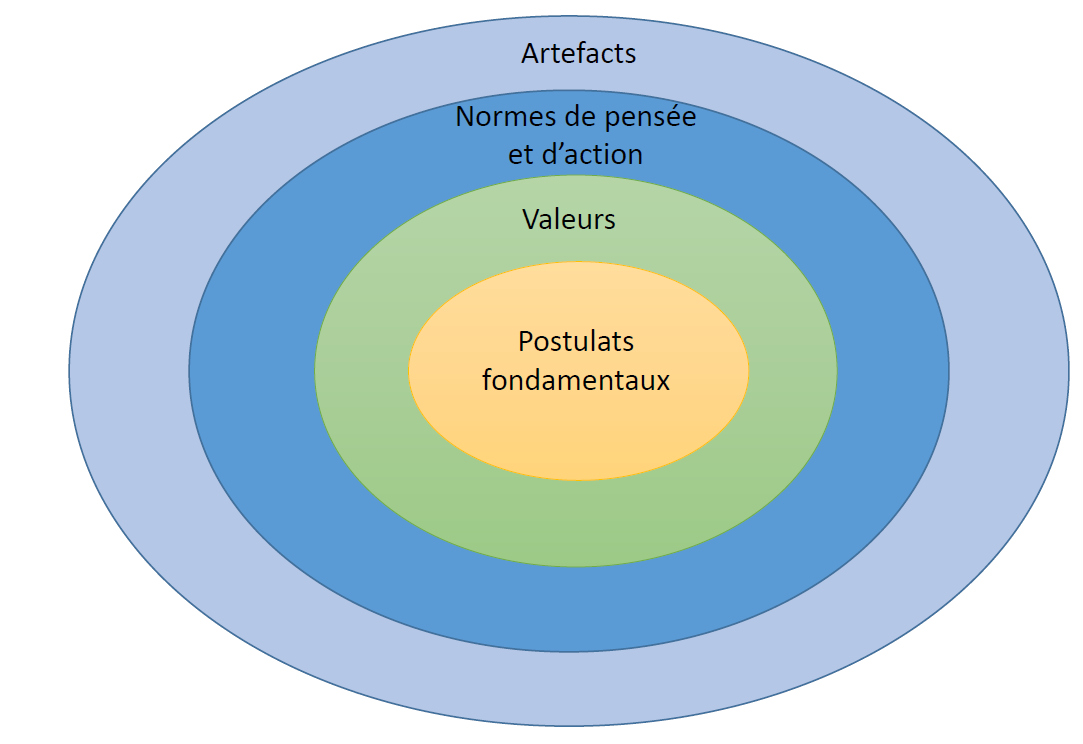
\includegraphics[width=\linewidth]{culture_orga_niveaux.png}
	  \end{center}
	  Les \textbf{postulats fondamentaux} ou prémisses sont les croyances qui sont l'essence de la culture. Ces prémisses sont difficiles à discerner car elles opèrent au niveau de l'inconscient. Elles portent sur des questions telles que la nature de l'homme, le rapport au temps, la notion de vérité, etc. Elles ne sont quasiment jamais remises en cause.
	  
	  Les artéfacts découlent des valeurs et les valeurs découlent des postulats fondamentaux.
	  
	  \end{multicols}
	  
      \subsection{Le modèle des valeurs concurrentes de Quinn}
	Ce modèle a été développé à l'origine pour décrire les valeurs sous-jacentes aux critères d'efficacité organisationnelle.
	
	Il caractérise les cultures organisationnelles selon 2 dimensions : le contrôle VS la flexibilité et les relations (interne) VS les résultats (externe).
	
	\subsubsection{Un phénomène multi-dimensionnel}
	
	  Quinn définit 4 grands types de cultures :
	  
	  La \textbf{culture de soutien} qui privilégie la coopération, la participation, l'attachement à l'entreprise, la communication interpersonnelle. C'est une culture de \og{} collaborateurs \fg{} qui peut se retrouver notamment dans les PME familiales.
	  
	  La \textbf{culture des règles} qui est très respectueuse des procédures, tout est écrit, tracé, standardisé. La communication est essentiellement descendante dans l'organigramme, c'est une culture \og{} d'organisateurs \fg{}. Cette culture peut se retrouver dans les administrations publiques.
	  
	  La \textbf{culture des buts} privilégie les objectifs de performance et la rationalisation des processus en vue des objectifs. C'est une culture de \og{} compétiteurs \fg{}. 
	  
	  La \textbf{culture de l'innovation} qui privilégie la créativité, l'ouverture au changement, l'expérimentation et l'adaptation permanente. La communication est aussi peu formalisée que possible pour casser la hiérarchie stricte, c'est une culture \og{} d'innovateurs \fg{}.
	  
	  Ce modèle peut se superposer à celui d'Ulrich pour tracer un historique des pratiques de ressources humaines.
	
	\subsection{La théorie des dimensions culturelles (1991)}
	
	Une organisation (de taille conséquente) n'est pas liée à une seule culture, il existe des sous-cultures. Il y a les sous-cultures par département, par métiers, par âge, par affinités,...
	
	  \subsubsection{Un phénomène hétérogène}
	  
	  Le modèle de Hofstede a pour but d'étudier les interactions entre les cultures en fonction de certaines dimensions en leur attribuant des scores de 1 à 120.
	  
	  Il met en avant 4 dimensions :
	  
	  \begin{enumerate}
	   \item Distance au pouvoir
	   \item Evitement de l'incertitude
	   \item Masculinité contre féminité
	   \item Individualisme contre collectivisme
	  \end{enumerate}
	  
	  La \textbf{distance au pouvoir} est un indice d'acceptation de pas avoir de pouvoir par les membres les plus éloignés de la direction dans l'organigramme.
	  Un indice faible signifie que les membres souhaitent une gestion démocratique et se considèrent à égalité avec les autres, un indice élevé indique que ceux qui ont le moins de pouvoir acceptent leur condition et sont forts soumis au pouvoir.
	  
	  L'\textbf{évitement de l'incertitude} correspond au degré de tolérance d'une société pour l'incertitude/l'ambiguité. Les sociétés avec un indice faible sont ouvertes aux changements, disposent de moins de règles et de lois et les directives y sont plus souples.
	  
	  La \textbf{masculinité contre la féminité} correspond au niveau d'importance accordée aux valeurs masculines (assurance, ambition, pouvoir, matérialisme) et aux valeurs féminines (égalité, relations humaines).
	  
	  L'\textbf{individualisme contre le collectivisme} correspond au degré auquel les individus sont intégrés aux groupes. Une culture individualiste donne de l'importance à l'initiative privée et la réussite d'objectif personnels, une culture collectiviste met en avant le bien-être du groupe, la loyauté, l'intérêt collectif avant l'intérêt personnel.
	  
	  Il est possible de croiser les dimensions entre elles.
	  
	  L'analyse pour la culture belge pourrait donner ceci : une distance au pouvoir plutôt forte, un évitement de l'incertitude fort, une légère prédominance masculine et une culture plutôt individualiste.
	  
	  \begin{figure}[!ht]
	   \begin{center}
	    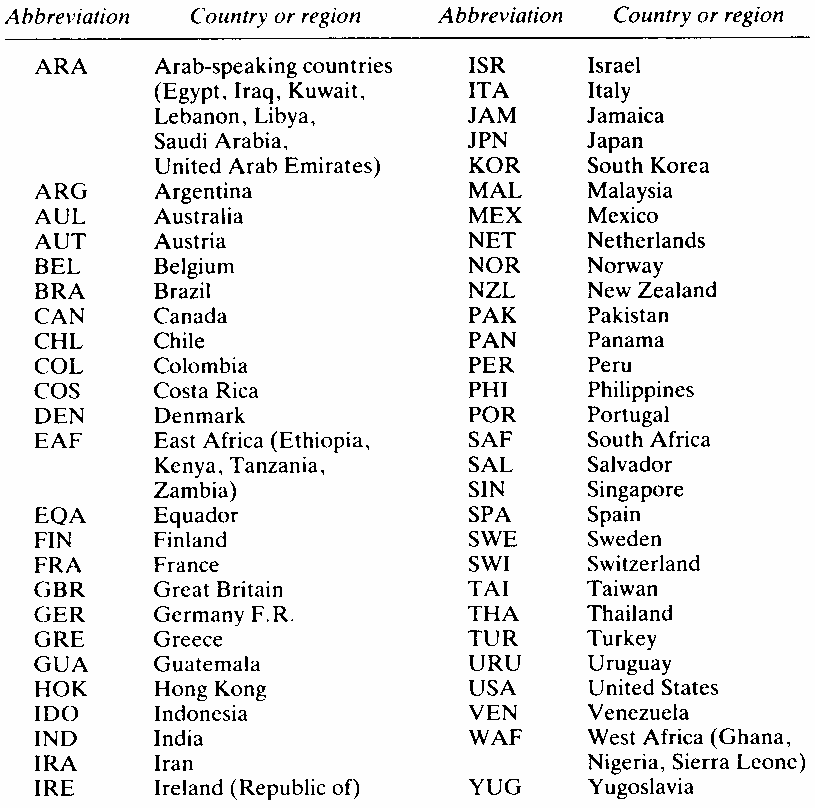
\includegraphics[width=0.65\linewidth]{hofstede_abbr.png}
	    \caption{Abréviations pour les pays et régions étudiés}
	   \end{center}
	  \end{figure}
	  
	  \begin{figure}[!ht]
	   \begin{center}
	    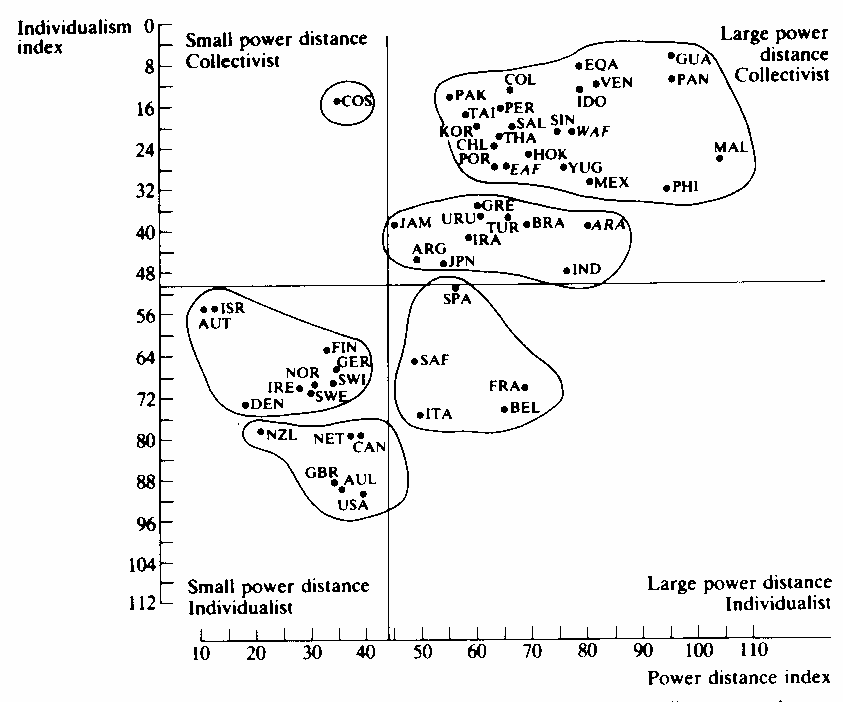
\includegraphics[width=0.65\linewidth]{hofstede_indivi_collect.png}
	    \caption{Position des 50 pays et 3 régions sur la distance au pouvoir et l'individualisme-collectivisme}
	   \end{center}
	  \end{figure}
	  
	  \begin{figure}[!ht]
	   \begin{center}
	     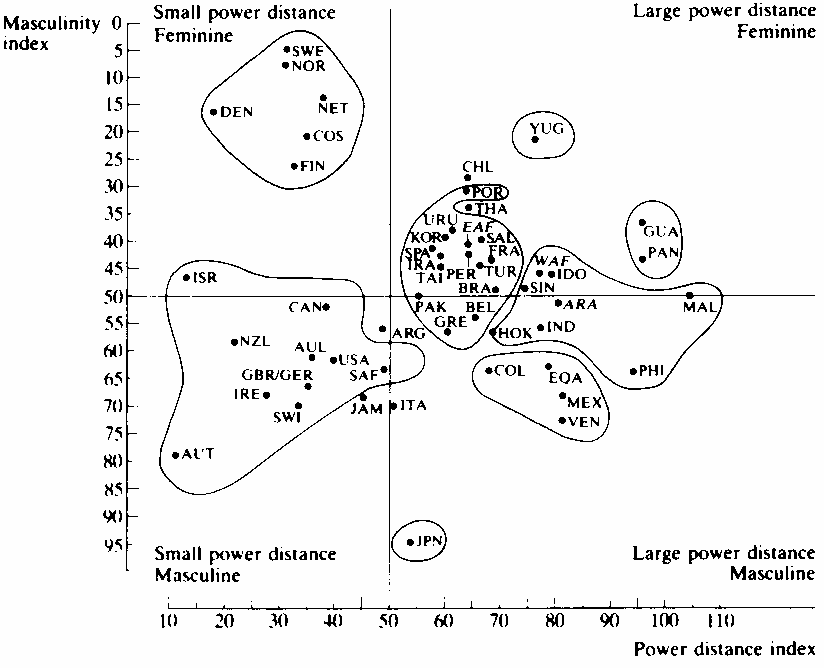
\includegraphics[width=0.65\linewidth]{hofstede_power_masc.png}
	     \caption{Distance au pouvoir contre masculinité pour 50 pays et 3 régions}
	   \end{center}
	  \end{figure}

	  \begin{figure}[!ht]
	   \begin{center}
	     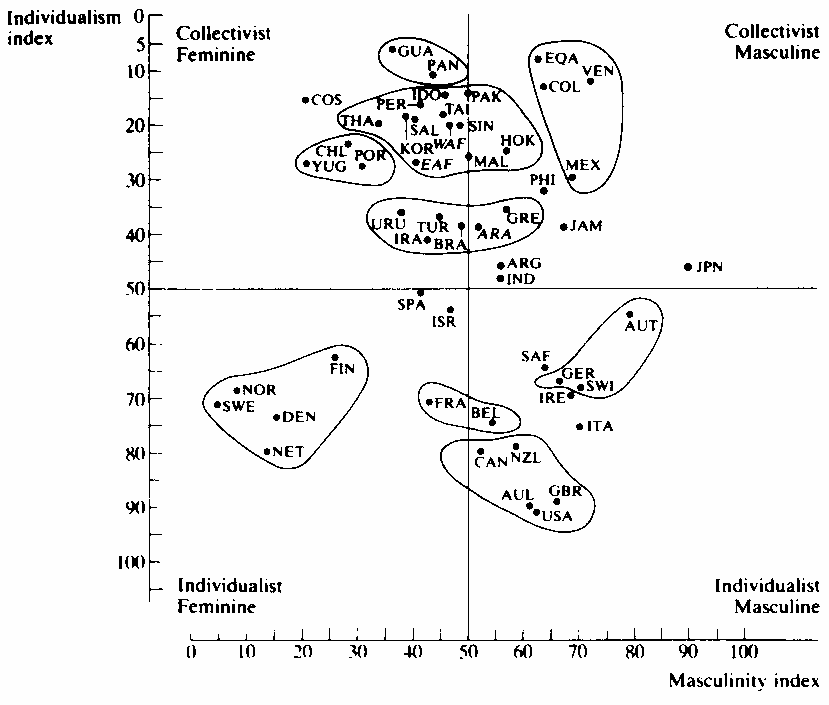
\includegraphics[width=0.65\linewidth]{hofstede_masc_indivi.png}
	     \caption{Position de 50 pays et 3 régions sur les dimensions masculinité-féminité et individualisme-collectivisme}
	   \end{center}
	  \end{figure}
	  
	  \begin{figure}[!ht]
	   \begin{center}
	    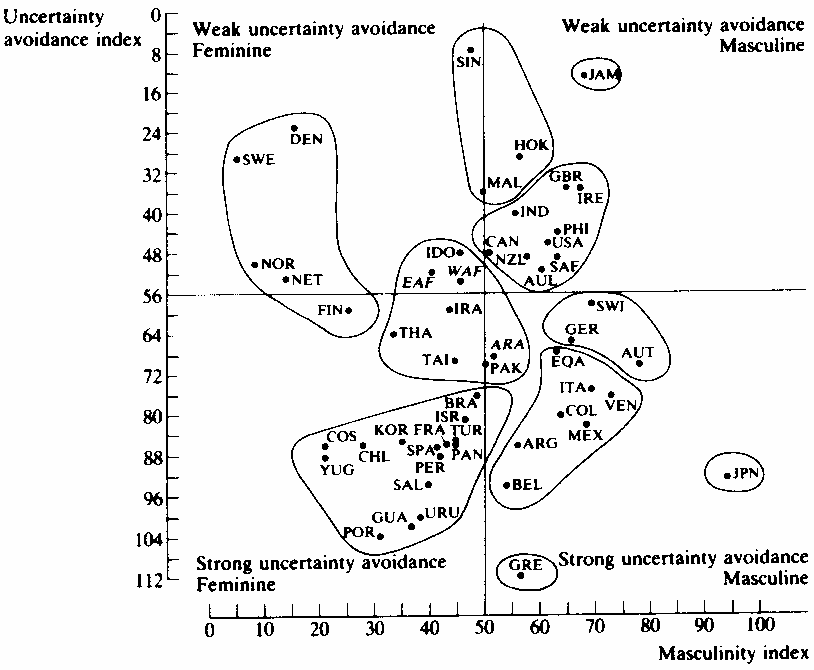
\includegraphics[width=0.65\linewidth]{hofstede_masc_incertitudes.png}
	    \caption{Position de 50 pays et 3 régions sur les dimensions masculinité/féminité et évitement de l'incertitude}
	   \end{center}
	  \end{figure}
	  
	  \begin{figure}[!ht]
	   \begin{center}
	    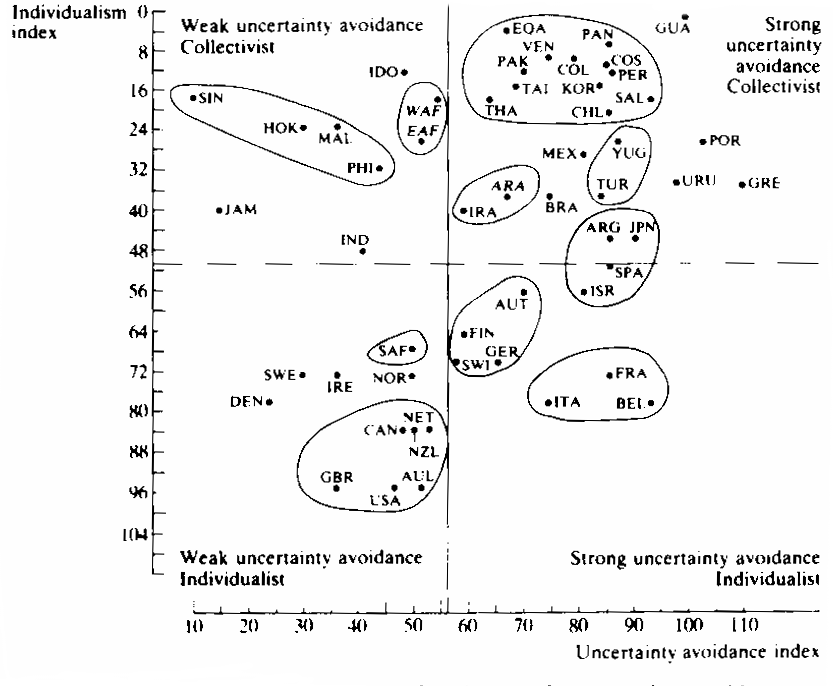
\includegraphics[width=0.65\linewidth]{hofstede_incertitudes_indivi.png}
	    \caption{Position de 50 pays et 3 régions sur les dimensions d'évitement d'incertitude et individualisme-collectivisme}
	   \end{center}
	  \end{figure}

	  \FloatBarrier % Force les flottants à se placer ici


	\subsection{Le cycle de perpétuation culturelle (Sathé, 1985)}
		\subsubsection{Un phénomène dynamique}
	\subsection{Les composantes de la culture organisationnelle (Thévenet)}
	\subsection{Méthodologies d'étude}
		\subsubsection{Type de culture et performance}
		\subsubsection{Culture et réactions individuelles}
		\subsubsection{Type de culture et réactions individuelles}
		\subsubsection{Adéquation individu-organisation et réactions individuelles}
		\subsubsection{Conclusion}
		
\section{Dynamique de groupe}
	\subsection{Le groupe dans l’histoire de l’organisation}
	
	La vision qu'on s'est faite du groupe a fortement évolué dans le temps: \newline
	
	Dans l'\textbf{Organisation Scientifique du Travail}, le groupe était perçu comme quelque chose de nuisible par le manager. Le but du Taylorisme est d'atomiser les groupes pour qu'ils n'existent pas. Les groupes formés étaient soit informel, soit alors clandestin. Cette vision perdure jusqu'à l'École des Relations Humaines.\newline
	
	Avec l'\textbf{École des Relations Humaines}, on remarque que le groupe peut avoir des effets bénéfiques. On commence à s'intéresser au bien-être qui impacte fortement l'efficacité. On considère le groupe comme quelque chose de positif. Il est conçu comme une source d'appartenance, de motivation et de conformisme.\newline
	
	Puis vient le \textbf{Courant Socio-Technique} avec qui on remarque que les changements techniques peuvent avoir de graves conséquences sur les relations humaines. L'équipe est alors très importante pour le changement.\newline
	
	Et enfin arrive l'\textbf{Entreprise Flexible} qui se caractérise par une gestion plus flexible des équipes. On met ensemble des experts pour travailler sur un projet (équipes projets ad hoc).
	
	\subsection{Définitions et types}
		\subsubsection{Définition}
		
		Le \textbf{groupe} est un \textit{ensemble} de 2 individus ou plus, \textit{interdépendants} dans la poursuite d'un \textit{but} identique. \newline
		
		Il est caractérisé par:
		\begin{itemize}
		\item Système social perçu comme une entité: il y une frontière entre les membres et les non-membres.
		\item Système social structuré et différencié: mécanisme de coordination.
		\item Interdépendance dans la réalisation d'une ou plusieurs tâches: certaines tâches ne sont pas réalisables sans les autres membres du groupe.
		\item Système ouvert sur son environnement: l'environnement (personnes en dehors du groupe) a un impact sur le travail du groupe.
		\end{itemize}
		
		\subsubsection{Types}
		
		%TODO ajouter les fléches des slides page 7 et 8
		On peut distinguer les groupes selon leur \textit{objectif} et la façon dont les \textit{interdépendances} sont structurés.	A partir de cela, on obtient 2 groupes: \newline
		
		Le \textbf{groupe informel} qui n'a pas de structure formellement définie par l'organisation. Ces groupes ne sont pas négligeables. C'est à l'intérieur de ces groupes que se transmettent les rumeurs,... De plus, s'ils ne sont composés d'aucun employés travaillant ensemble, on peut supposer qu'il y a des soucis (surtout vrai pour les groupes d'affinités). Le groupe informel peut lui-même être subdivisé en 2 catégories:
		\begin{itemize}
		\item \textbf{Groupe d'affinité} qui sont des personnes se réunissant pour partager un ou plusieurs points communs.\newline 
		ex:Personnes qui courent ensemble.
		\item \textbf{Groupe d'intérêt} qui sont des personnes travaillant ensemble pour atteindre un objectif spécifique.\newline 
		ex:Employés qui se rassemblent pour une pétition suite au licenciement d'un collègue. \newline
		\end{itemize}
		
		Le \textbf{groupe formel} est un groupe de travail déterminé par la structure de l'entreprise. Le groupe formel peut lui aussi être subdivisé en 2 catégories:
		\begin{itemize}
		\item Le \textbf{groupe hiérarchique} est groupe composé d'individus qui se réfèrent directement à un responsable déterminé.
		\item Le \textbf{groupe de travail} est un ensemble de personnes travaillant ensemble afin de réaliser une tâche ou un projet spécifique. Dans ce type de groupe de travail, on ne se réfère pas forcément à un supérieur. Il est possible d'en choisir un pour le projet seulement.\newline
		ex: Parents, professeurs et le directeur qui se réunissent pour discuter de l'expulsion d'un élève. Chaque personne emmène son expertise. Il n'y a pas de vrai hiérarchie. \newline
		\end{itemize}
		
		On peut aussi diviser les équipes de travail selon l'\textit{empowerment} ( dans quelle mesure les équipes disposent de pouvoir pour se strucuture):
		\begin{itemize}
		\item \textbf{Traditionnelles} qui est sous la direction d'un supérieur (organigramme).
		\item \textbf{Consultatives} dont les membres de l'équipe peuvent proposer des solutions mais la décision finale revient au chef. \newline
		ex: Cercles de qualité.
		\item \textbf{Ad hoc} qui sont des groupes de projets ponctuels. Ils disposent d'une marge de man\oe uvre pour leur structuration.
		\item \textbf{Semi-autonomes} qui sont des équipes de travail ayant un but de production mais disposant d'une liberté de gestion. 
		\end{itemize}
		
		
	\subsection{Dynamique des groupes restreints}
	
	Un \textbf{groupe restreint} est un groupe disposant d'un nombre de membres réduit (inférieur à 20).
	%TODO trouver définition de dynamique des groupes
	
		\subsubsection{Anzieu et Martin (1968)}
	
			
		
		\subsubsection{Les étapes de la vie d’un groupe (Tuckman, 1965)}
		
		Les groupes se constituent. Ils passent par différentes étapes : \newline
		%Film "Remember the titans"
		\begin{itemize}
		\item \textbf{Formation} (ou constitution): durant cette étape on travaille la \textit{confiance}. On ne connaît pas les autres membres du groupe, leurs normes, .... On essaye dès lors d'observer comment le groupe agit mais en gardant une certaine distance. On est en pleine incertitude. Cette étape se termine quand on sent qu'on appartient au groupe.
		\item \textbf{Agitation}: c'est l'étape de \textit{structuration des tâches et des rôles} (pas simple et parfois lente). Il faut définir une hiérarchie. Cette période est également caractérisée par des conflits. Cette phase est importante et incontournable.
		\item \textbf{Normalisation}: on crée des \textit{normes} de fonctionnement et chaque membre doit y \textit{adhérer}. Les liens se renforcent. Il y a un sentiment d'appartenance. Cette étape se termine quand tout le monde sait comment se comporter.
		\item \textbf{Performance} (ou rendement): on se concentre sur la performance. Réalisation des buts et adaptation.
		\item \textbf{Dissolution}: fin du groupe. Peut être difficile pour certaines personnes. \newline
		\end{itemize}
		
		On peut toutefois porter certaines critiquer sur le modèle. En effet, le modèle est \textit{linéaire}. Tuckman suppose qu'on ne peut pas revenir à une étape antérieure. De plus, il ne tient pas compte du \textit{contexte} ou de l'\textit{environnement}. Dés fois, on doit être performant tout de suite ou bien certaines étapes sont faites à votre place (chef, normes, ... définis déjà par l'organisation par exemple). \newline
		
		On a remarqué que ces groupes se remettent en question au même moment.\newline
		%TODO schéma montrant performance en fonction du temps		
		
		Il existe aussi une dynamique des \textbf{groupes temporaires}.\newline
		ex: Un groupe formé pour 2h seulement. \newline
		
				
		\subsubsection{Cohésion affective}
		
		La \textbf{cohésion affective} est le degré d'\textit{attractivité} des membres les uns pour les autres.	\newline
		
		Elle est fonction de l'\textit{homogénéité} du groupe. Un groupe composé de personnes similaires ayant plusieurs points communs aura une meilleure cohésion. Elle accroît la \textit{satisfaction} et renforce le \textit{conformisme}. Toutefois, la cohésion affective est \textbf{faiblement corrélé à la performance}. Une grande cohésion peut emmener tout les membres du groupe à prendre la même décision qui est la mauvaise. \newline
		
		On peut analyser la cohésion affective d'un groupe ou organisation à l'aide d'un \textbf{sociogramme}. \newline 
		
		Un sociogramme est un diagramme des liens sociaux qu'une personne possède. Les critères qui servent à établir un tel diagramme sont divers: relations personnelles, relations professionnelles, canaux de communication, .... Cet outil permet d'objectiver la dynamique des groupes, afin qu'un animateur ou un enseignant, par exemple, soient moins influencés par leurs sentiments et leurs préjugés lorsqu'ils établissent des équipes de travail.\newline
		%TODO schéma sociogramme
		
		
		\subsubsection{Facteurs de cohésion d’un groupe}
		
		%TODO reprendre schéma des slides
		
				
		\subsubsection{Structuration des rôles et statuts}
		
		Les \textbf{rôles} sont un ensemble d'attitudes et comportements attendus de celui qui occupe une position dans un groupe. \newline 
		%TODO trouver une meilleure phrase
		Plusieurs catégories par rapport au rôle:
		\begin{itemize}
		\item \textbf{Attentes de rôles}: du fait qu'on occupe un rôle bien déterminé, les autres membres (ou même des extérieures au groupe) peuvent avoir certaines attentes par rapport à toi. Parfois des attentes non fondées. Il y a donc risque de conflits et d'ambiguïtés de rôles.
		\item \textbf{Identité de rôle}: attitudes et comportements attendus du rôle. On peut changer aussi de rôle, identités multiples qui sont parfois conflictuelles. C'est la vision que se font les autres du rôles.
		\item \textbf{Perception de rôle}: idée qu'on se fait des attitudes et comportements à prendre du rôle qu'on occupe. Il y a risque de décalage entre attentes et perceptions. C'est la vision que moi, qui occupe le rôle, se fait justement de ce rôle. \newline
		\end{itemize}
		
		%TODO ajouter lien youtube.
		On peut illustrer la notion de rôle par l'\textbf{expérience de Zimbardo}(1971).C'est une étude  de  psychologie  expérimentale  sur  les  effets  de  la  situation  carcérale. Des  étudiants 
(sélectionnés  pour  leur  stabilité  et  leur  maturité) jouent  aléatoirement  le  rôle  de  gardiens  ou  de 
prisonniers. Cette expérience vise l’étude du comportement de personnes ordinaires dans un tel contexte, l’étude 
eut pour effet de montrer que c’est la \textbf{situation plutôt que la personnalité des participants qui était 
à l’origine de comportements parfois à l’opposé des valeurs professées par les participants avant 
l’étude}. Les étudiants agissent en fonction de leur rôle et non en fonction de leurs croyances. \newline

		Le \textbf{statut} est un ensemble d'attributs liés à la position d'un individu dans un système culturel donné. \newline
		
		On peut aussi définir le \textbf{statut} comme étant la place ou le rang occupé au sein d'un groupe et conférant un certain prestige.\newline
		
		Il existe \textbf{3} sources de statut. La première source est le \textbf{pouvoir exercé sur les autres}.	 La deuxième est la \textbf{capacité à contribuer aux objectifs du groupe}. Enfin, les dernières sont les \textbf{singularités propres à l'individu, valorisées par les groupe et le système culturel}. \newline
		
		Tout ceci influence le conformisme, les interactions et le sentiment d'équité. Une personne qui se conforme moins aux normes dispose souvent d'un statut plus élevé. De même, le fait de couper la paroles, se faire grand, ... sont les signes de quelqu'un qui occupe un statut privilégié (même si cela peut être négatif).
		
		\subsubsection*{Les 9 rôles d'équipiers de Belbin(1988)}		
		
		
		%Source belbinfrance.com		
		La \textbf{méthode Belbin} est un outil rationnel et rigoureux qui permet d'évaluer, de manière non intuitive, la coopération des membres d'une équipe. En identifiant les rôles endossés par chacun, on peut augmenter l'efficacité  des équipes en jouant, à bon escient , sur sa composition ou sur son fonctionnement interne.Il existe 9 rôles réparties en 3 catégories.\newline
		
		La \textbf{molécule de Belbin} illustre parfaitement le fait que les rôles se complémentent et que chaque rôle doit être présent dans l'équipe. \newline
		%TODO ajouter les schémas.
		\subsubsection{Normes, valeurs et conformisme}
		
				
		\subsubsection{La pensée de groupe (Janis, 1972)}
	\subsection{Le groupe, levier de changement}
	\subsection{Entreprise flexible : l’équipe de travail, lieu d’efficacité}
	\subsection{Le groupe de travail en pratique}
		
\section{Leadership}
	\subsection{Définitions et approches}
	\subsection{Distinctions conceptuelles : management \& leadership}
	\subsection{Approche axée sur les traits}
	\subsection{Approche axée sur les comportements}
	\subsection{Approchée axée sur la situation}
	\subsection{Retour à des approches personnalisantes}
	\subsection{Les conceptions du leadership dans leur contexte historique}

\section{La motivation au travail}
	\subsection{Définition}
	\subsection{Histoire}
	\subsection{Conception instrumentale de la motivation}
		\subsubsection{Principes du conditionnement}
		\subsubsection{En pratique…}
		\subsubsection{Effets de la conception instrumentale}
	\subsection{Conception humaniste de la motivation}
		\subsubsection{La pyramide de Maslow}
		\subsubsection{Le modèle bi-factoriel de Herzberg}
		\subsubsection{La théorie de McClelland}
		\subsubsection{La théorie ESC d’Alderfer (1969)}
		\subsubsection{En pratique… L’enrichissement du travail}
		\subsubsection{Effets de la conception humaniste}
	\subsection{Conception rationnelle de la motivation}
		\subsubsection{Les théories de processus}
		\subsubsection{Le modèle de room : la théorie des attentes}
		\subsubsection{En pratique}
		\subsubsection{Théorie de l’effet de but (Locke, 1968)}
		\subsubsection{Management by objectives (P. Drucker, 1954)}
		\subsubsection{Effet de la conception rationnelle}
	\subsection{Conception sociale de la motivation}
		\subsubsection{La théorie de l’équipe d’Adams}
		\subsubsection{En pratique}
		\subsubsection{Effets de la conception sociale}
		\subsubsection{Justice organisationnelle (Greenberg 1987)}
	\subsection{Et aujourd’hui…}
		Comment peut-on encore encourager la motivation et l’implication du personnel ?
		\subsubsection{Dans quel paysage travaillons-nous ?}
		\subsubsection{Formes traditionnelles du contrat psychologique}
		\subsubsection{Effets du contrat psychologique}
		\subsubsection{Formation et rupture du contrat psychologique}
		\subsubsection{Effets de la conception négociée}
		\subsubsection{En pratique…}
		\subsubsection{Que retenir ?}

\section{Conclusion}

\bibliographystyle{plain}
\bibliography{biblio}


\end{document}
